\chapter{Project Specification}
\section{Functional Requirements}
\begin{itemize}
    \item The project must involve the selection of publicly available health-related datasets
    \item The project must begin by pre-processing and exploratory data analysis
    \item The project must use Random Forest as an algorithm to create models to fit the various datasets.
    \item The project must record performance metrics as a baseline
    \item The project must use random under-sampling of the majority class in varying proportions.
    \item The project must use over-sampling of the minority class with appropriate parameters for the datasets 
    \item The performance metrics obtained in the different situations must be compared to the baseline
\end{itemize}

\section{Non-Functional Requirements}
\begin{itemize}
    \item The project will use R as a language to carry out the analysis
    \item The project will use the necessary available library and package of R for Random Forest and graph generation
    \item The project will use SSPS for statistical analysis
\end{itemize}

\chapter{Project Management}
The project management for this project was done using GitHub as both a version control tool and a project management tool. The KanBan-style boards allowed for the creation of milestones, tasks and issues to help keep track of the coding portion of the project and for the thesis writing part of the project.\newline
Since a GitHub interface was not constantly open while working on the project, it was relatively frequent to forget to mark a task or milestone as completed, although the version control was always carried out and both code and thesis were frequently updated.\newline
A GitHub repository was created for the actual analysis and coding tasks and a separate one was created to keep track of  the various deadlines and milestones for the thesis writing.\newline
Weekly meeting were also set up with my supervisor to discuss on-going work, results, potential issues and progress on the project.\newline
Coursework hand-in weeks and other deadlines from other modules were on occasion conflicting with due deadlines and milestone for the project and this caused stress, particularly in semester 1.

\chapter{Implementation Appendix}

\begin{figure}[!htbp]
    \centering
    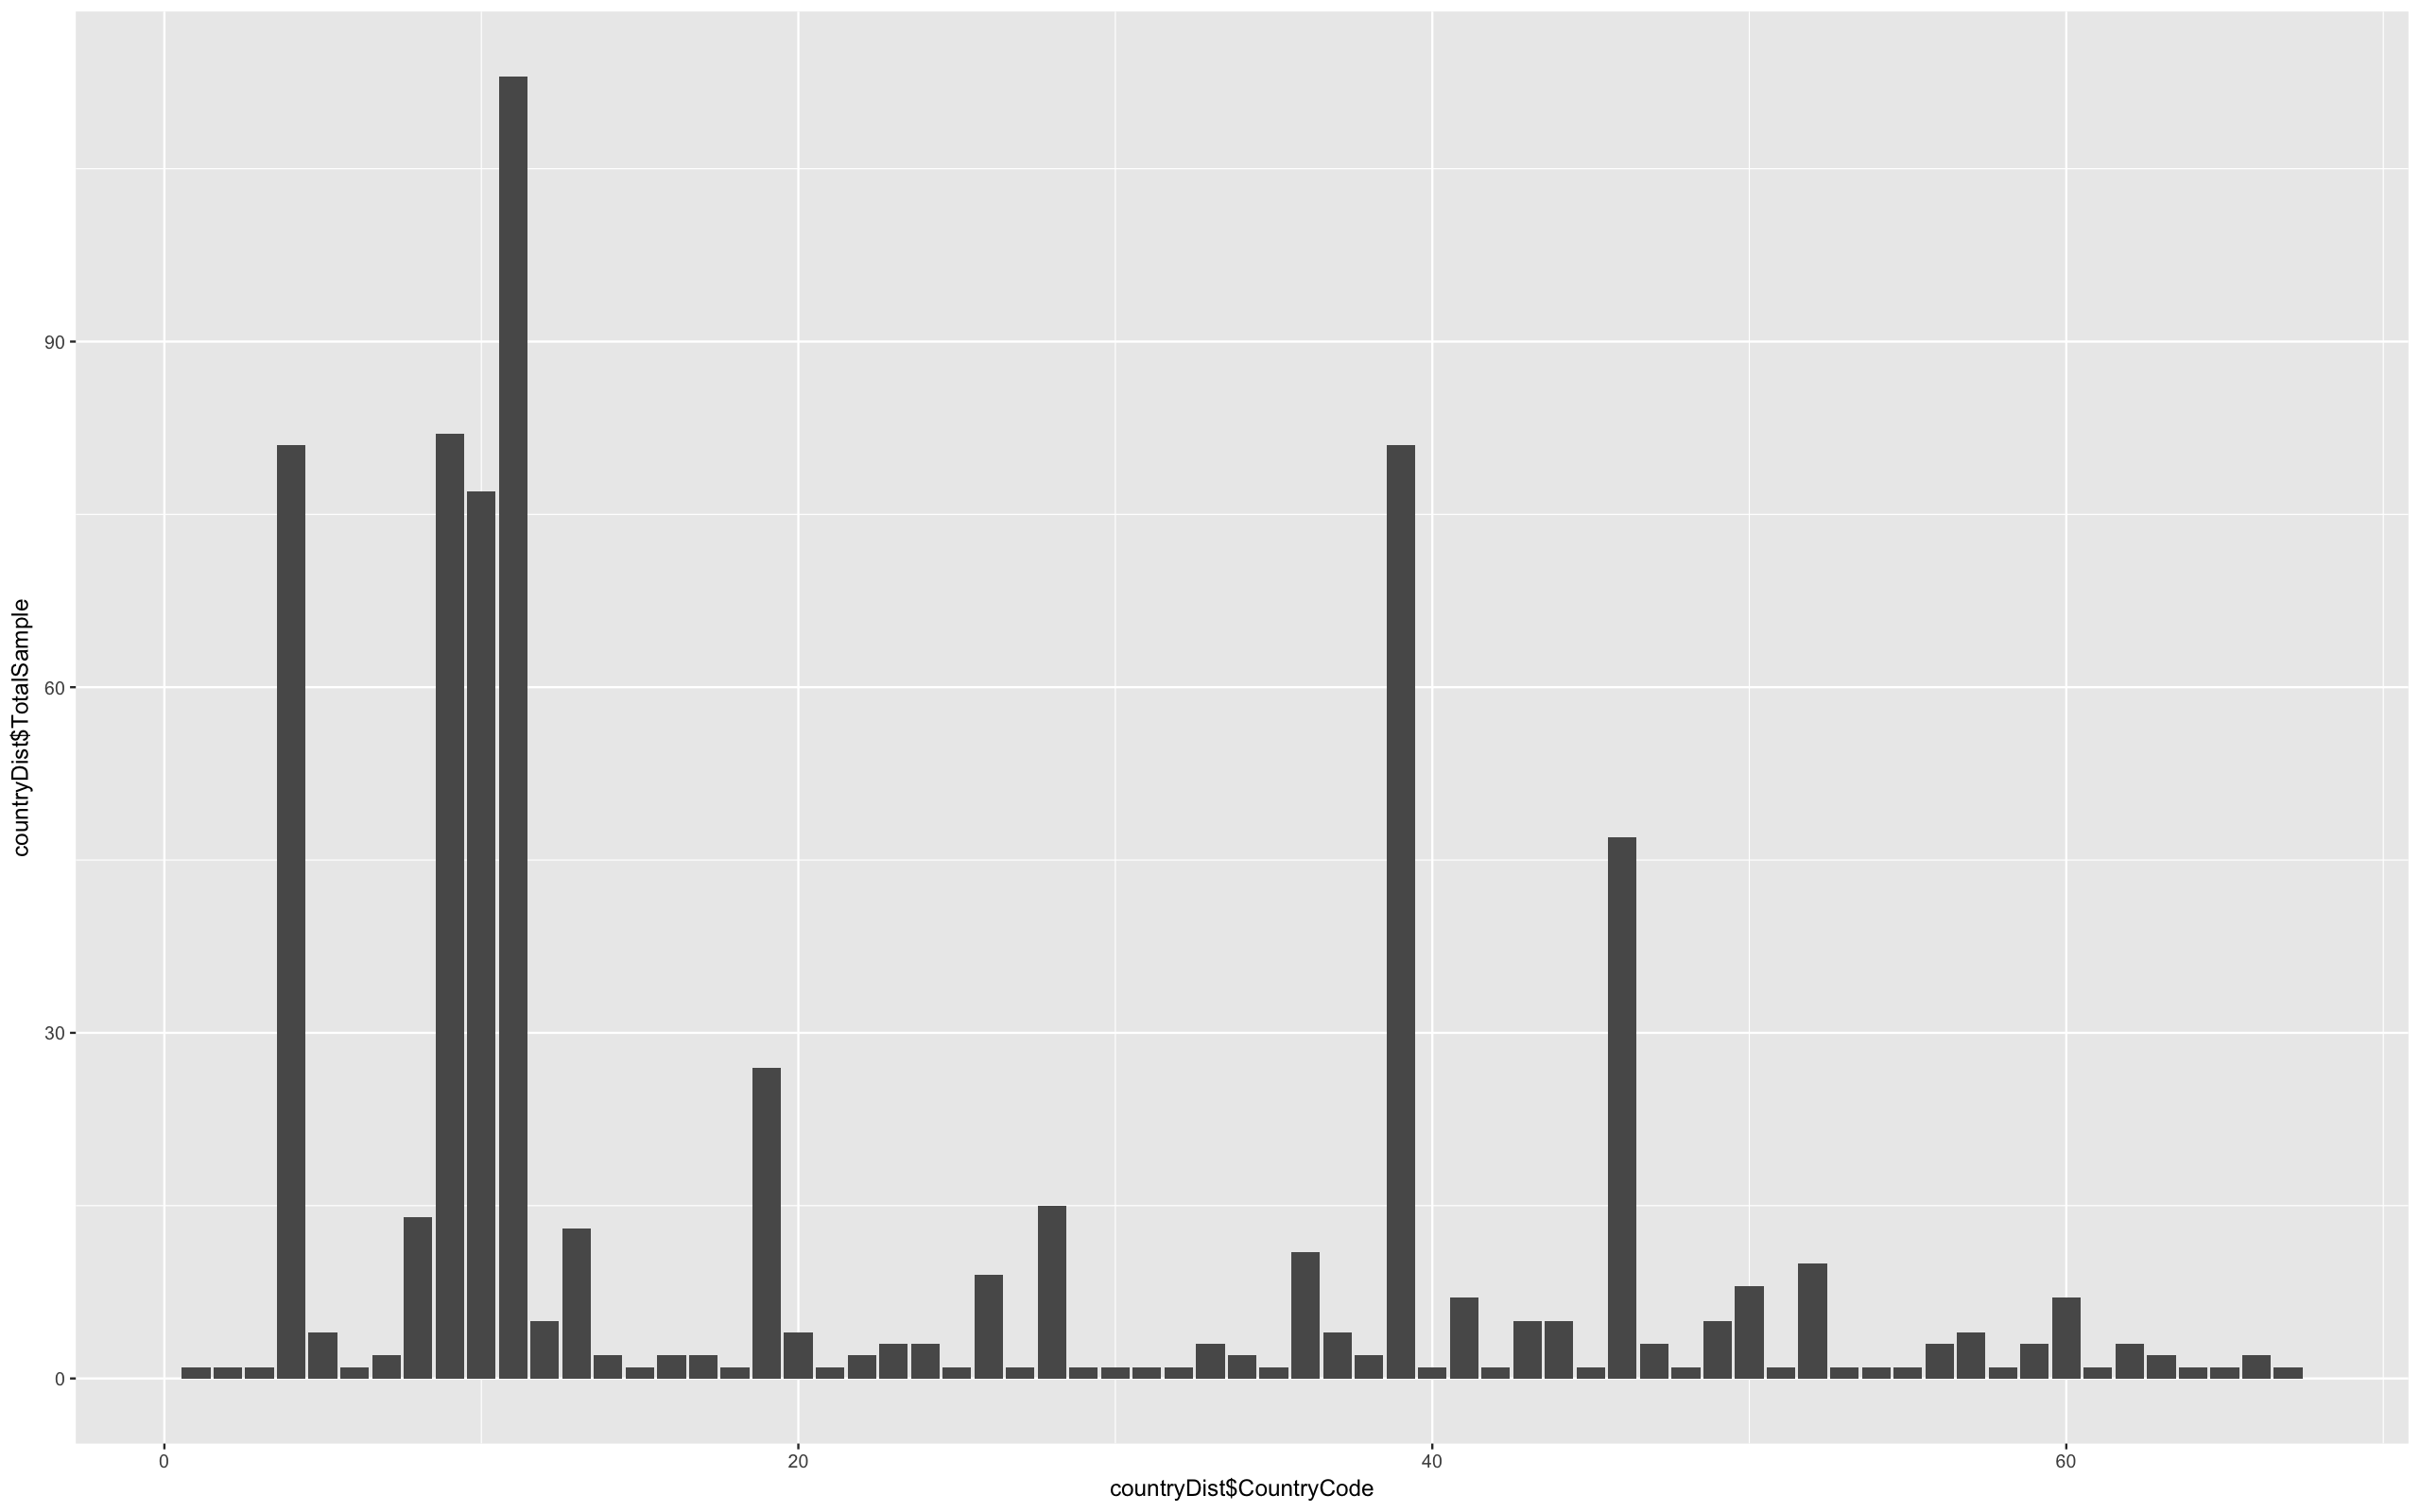
\includegraphics[width=0.9\textwidth]{ThesisTemplate/appendix/images/figure4_2b.png}
    \caption{Distribution of the autism data by country of residence.}
    \label{fig:Autism Distribution}
\end{figure}

\chapter{Evaluation Appendix}
\begin{figure}[!htbp]
    \centering
    \begin{minipage}{0.45\textwidth}
        \centering
        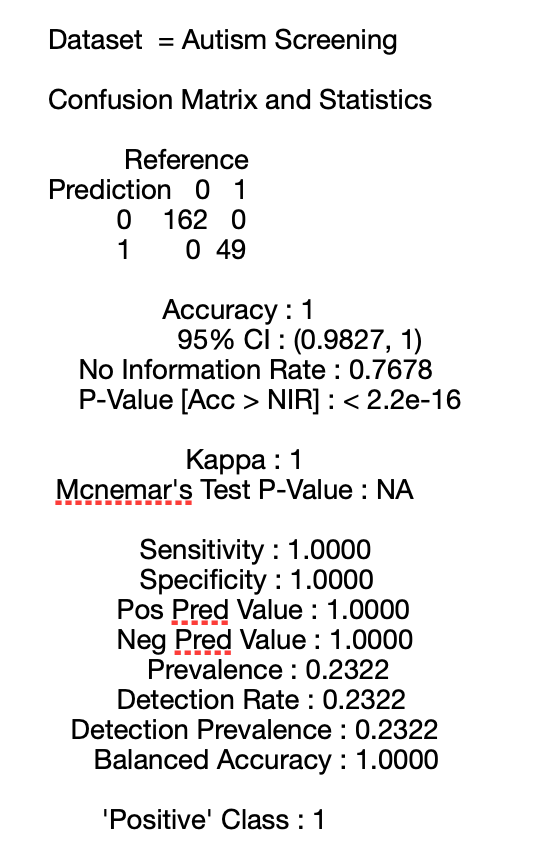
\includegraphics[width=0.9\textwidth]{ThesisTemplate/appendix/images/Chapter5Appendix/ConfusionMatrix/Autism.png} 
        \caption{Confusion Matrix output for Random Forest fitted to the Autism Dataset}
        \label{fig:matrixAutism}
    \end{minipage}\hfill
    \begin{minipage}{0.45\textwidth}
        \centering
        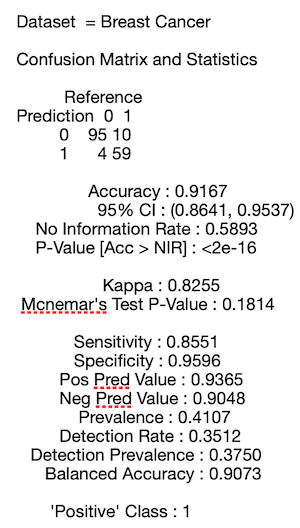
\includegraphics[width=0.9\textwidth]{ThesisTemplate/appendix/images/Chapter5Appendix/ConfusionMatrix/BreastCancer.png} 
        \caption{Confusion Matrix output for Random Forest fitted to the Breast Cancer Dataset}
        \label{fig:matrixBC}
    \end{minipage}
\end{figure}

\begin{figure}[!htbp]
    \centering
    \begin{minipage}{0.45\textwidth}
        \centering
        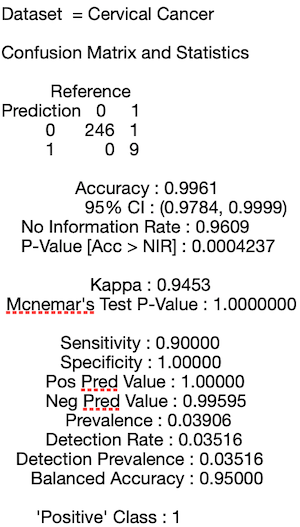
\includegraphics[width=0.9\textwidth]{ThesisTemplate/appendix/images/Chapter5Appendix/ConfusionMatrix/CervicalCancer.png} 
        \caption{Confusion Matrix output for Random Forest fitted to the Cervical Cancer Dataset}
        \label{fig:matrixCC}
    \end{minipage}\hfill
    \begin{minipage}{0.45\textwidth}
        \centering
        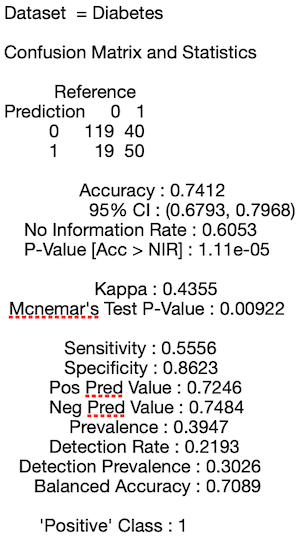
\includegraphics[width=0.9\textwidth]{ThesisTemplate/appendix/images/Chapter5Appendix/ConfusionMatrix/Diabetes.png} 
        \caption{Confusion Matrix output for Random Forest fitted to the Diabetes Dataset}
        \label{fig:matrixDia}
    \end{minipage}
\end{figure}

\begin{figure}[!htbp]
    \centering
    \begin{minipage}{0.45\textwidth}
        \centering
        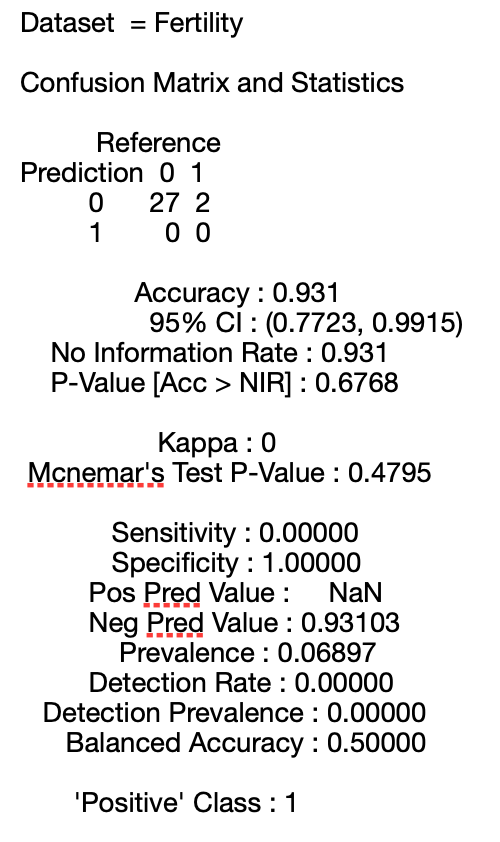
\includegraphics[width=0.9\textwidth]{ThesisTemplate/appendix/images/Chapter5Appendix/ConfusionMatrix/Fertility.png} 
        \caption{Confusion Matrix output for Random Forest fitted to the Fertility Dataset}
        \label{fig:matrixFert}
    \end{minipage}\hfill
    \begin{minipage}{0.45\textwidth}
        \centering
        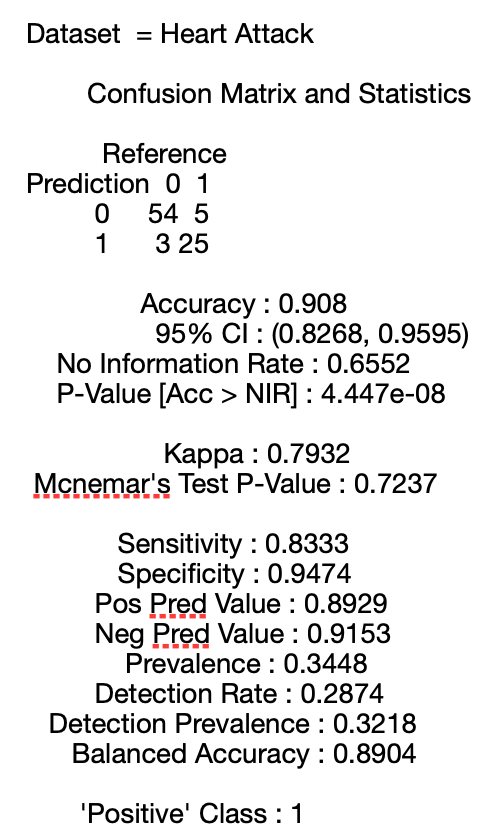
\includegraphics[width=0.9\textwidth]{ThesisTemplate/appendix/images/Chapter5Appendix/ConfusionMatrix/HeartAttack.png} 
        \caption{Confusion Matrix output for Random Forest fitted to the Heart Attack Dataset}
        \label{fig:matrixHA}
    \end{minipage}
\end{figure}


\begin{figure}[!htbp]
    \centering
    \begin{minipage}{0.45\textwidth}
        \centering
        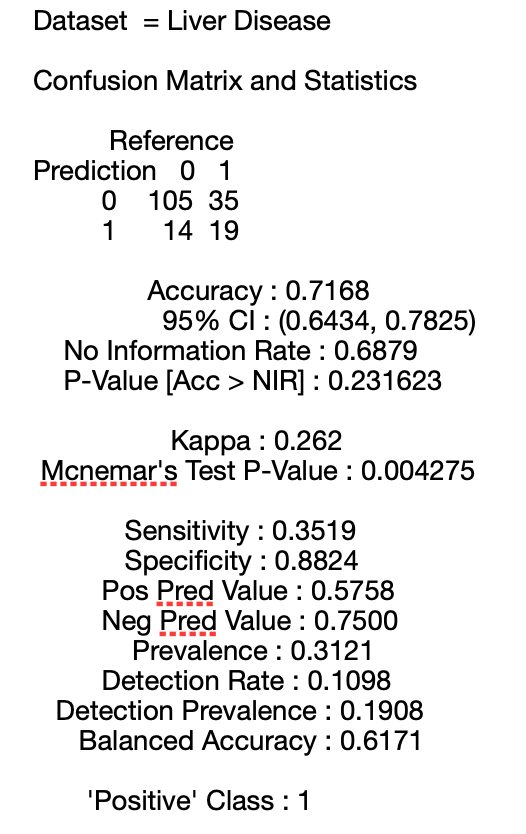
\includegraphics[width=0.9\textwidth]{ThesisTemplate/appendix/images/Chapter5Appendix/ConfusionMatrix/LiverDisease.png} 
        \caption{Confusion Matrix output for Random Forest fitted to the Liver Dataset}
        \label{fig:matrixLiver}
    \end{minipage}\hfill
    \begin{minipage}{0.45\textwidth}
        \centering
        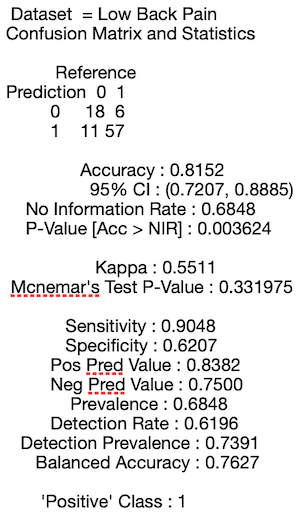
\includegraphics[width=0.9\textwidth]{ThesisTemplate/appendix/images/Chapter5Appendix/ConfusionMatrix/LowBackPain.png} 
        \caption{Confusion Matrix output for Random Forest fitted to the Low Back Pain Dataset}
        \label{fig:matrixLBP}
    \end{minipage}
\end{figure}

\begin{figure}[!htbp]
    \centering
    \begin{minipage}{0.45\textwidth}
        \centering
        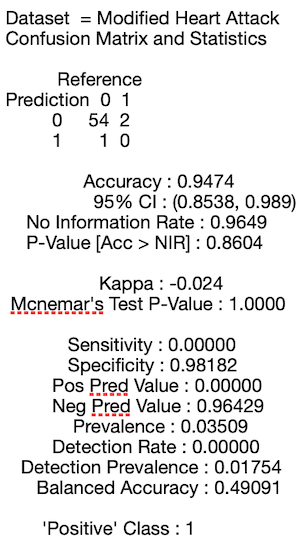
\includegraphics[width=0.9\textwidth]{ThesisTemplate/appendix/images/Chapter5Appendix/ConfusionMatrix/modHeartAttack.png} 
        \caption{Confusion Matrix output for Random Forest fitted to the Modified Heart Attack Dataset}
        \label{fig:matrixmodHA}
    \end{minipage}\hfill
    \begin{minipage}{0.45\textwidth}
        \centering
        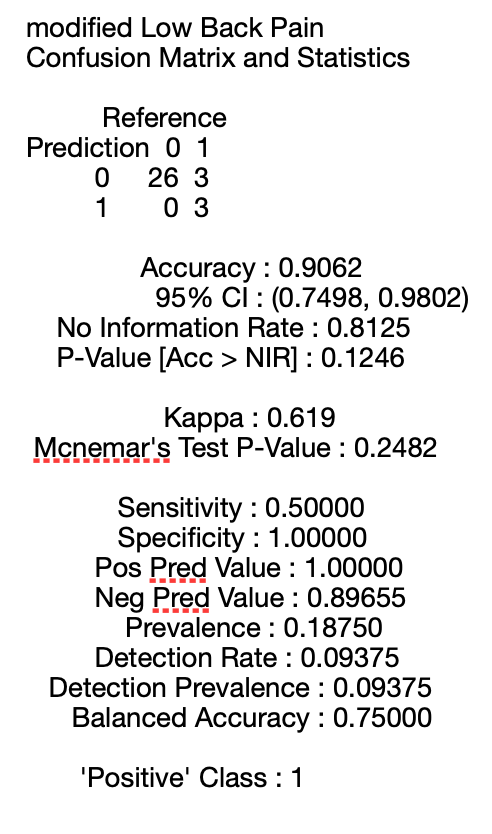
\includegraphics[width=0.9\textwidth]{ThesisTemplate/appendix/images/Chapter5Appendix/ConfusionMatrix/modLowBackPain.png} 
        \caption{Confusion Matrix output for Random Forest fitted to the Modified Low Back Pain Dataset}
        \label{fig:matrixmodLBP}
    \end{minipage}
\end{figure}


\begin{figure}[!htbp]
    \centering
    \begin{minipage}{0.45\textwidth}
        \centering
        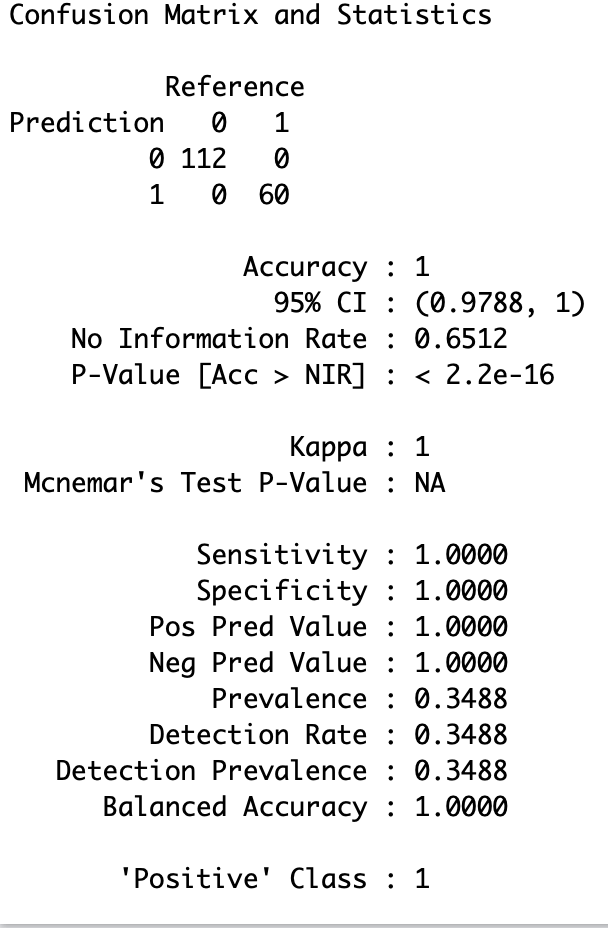
\includegraphics[width=0.9\textwidth]{ThesisTemplate/appendix/images/Chapter5Appendix/ConfusionMatrix75/Autism.png}
        \caption{Confusion Matrix output for Random Forest fitted to the Autism Dataset after under-sampling (75\% majority class retained)}
        \label{fig:my_label}
    \end{minipage}\hfill
    \begin{minipage}{0.45\textwidth}
        \centering
        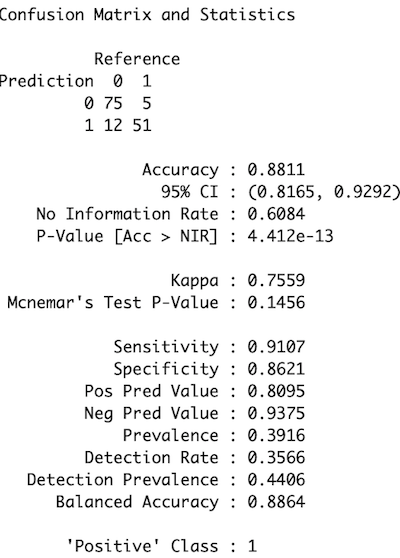
\includegraphics[width=0.9\textwidth]{ThesisTemplate/appendix/images/Chapter5Appendix/ConfusionMatrix75/BreastCancer.png}
        \caption{Confusion Matrix output for Random Forest fitted to the Breast Cancer Dataset after under-sampling (75\% majority class retained)}
        \label{fig:matrixAutism75}
    \end{minipage}
\end{figure}

\begin{figure}[!htbp]
    \centering
    \begin{minipage}{0.45\textwidth}
        \centering
        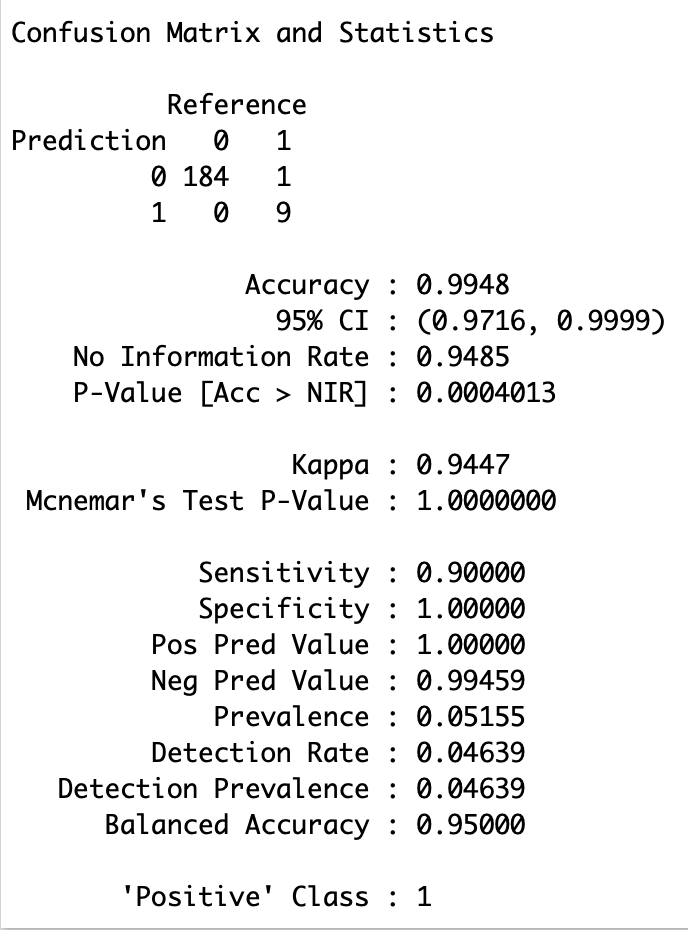
\includegraphics[width=0.9\textwidth]{ThesisTemplate/appendix/images/Chapter5Appendix/ConfusionMatrix75/CervicalCancer.png}
        \caption{Confusion Matrix output for Random Forest fitted to the Cervical Cancer Dataset after under-sampling (75\% majority class retained)}
        \label{fig:matrixCC75}
    \end{minipage}\hfill
    \begin{minipage}{0.45\textwidth}
        \centering
        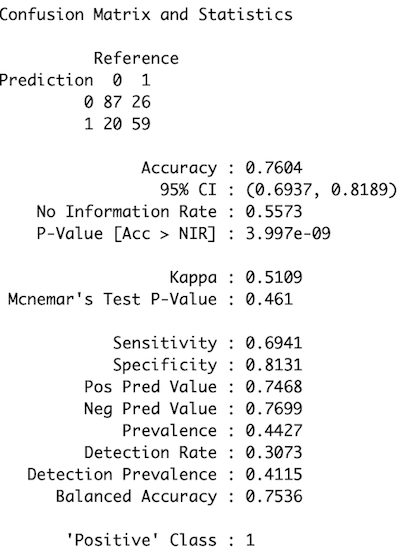
\includegraphics[width=0.9\textwidth]{ThesisTemplate/appendix/images/Chapter5Appendix/ConfusionMatrix75/Diabetes.png}
        \caption{Confusion Matrix output for Random Forest fitted to the Diabetes Dataset after under-sampling (75\% majority class retained)}
        \label{fig:matrixDia75}
    \end{minipage}
\end{figure}

\begin{figure}[!htbp]
    \centering
    \begin{minipage}{0.45\textwidth}
        \centering
        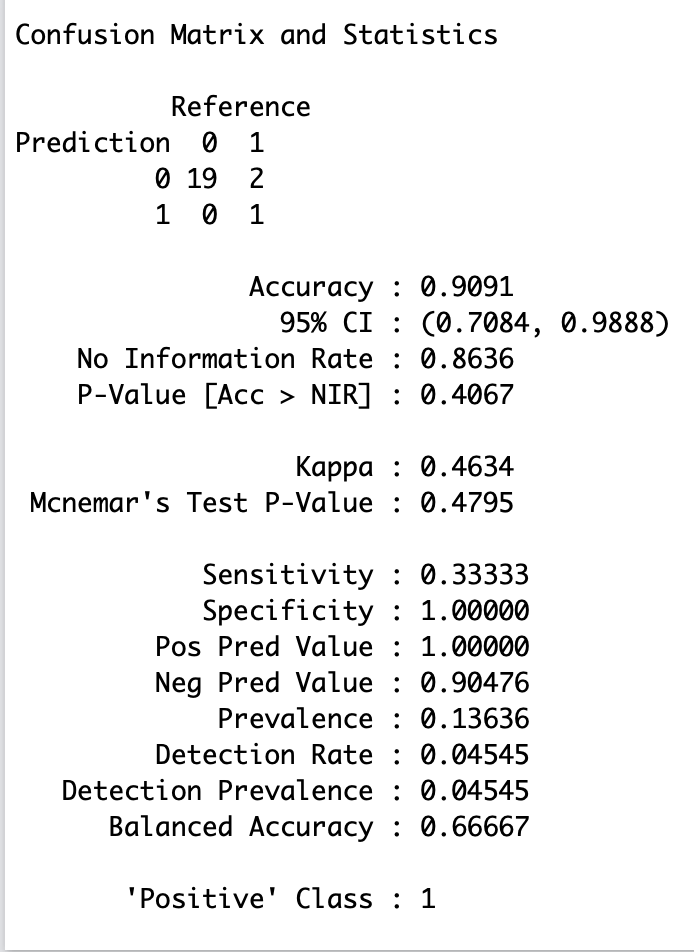
\includegraphics[width=0.9\textwidth]{ThesisTemplate/appendix/images/Chapter5Appendix/ConfusionMatrix75/Fertility.png}
        \caption{Confusion Matrix output for Random Forest fitted to the Fertility Dataset after under-sampling (75\% majority class retained)}
        \label{fig:matrixFert75}
    \end{minipage}\hfill
    \begin{minipage}{0.45\textwidth}
        \centering
        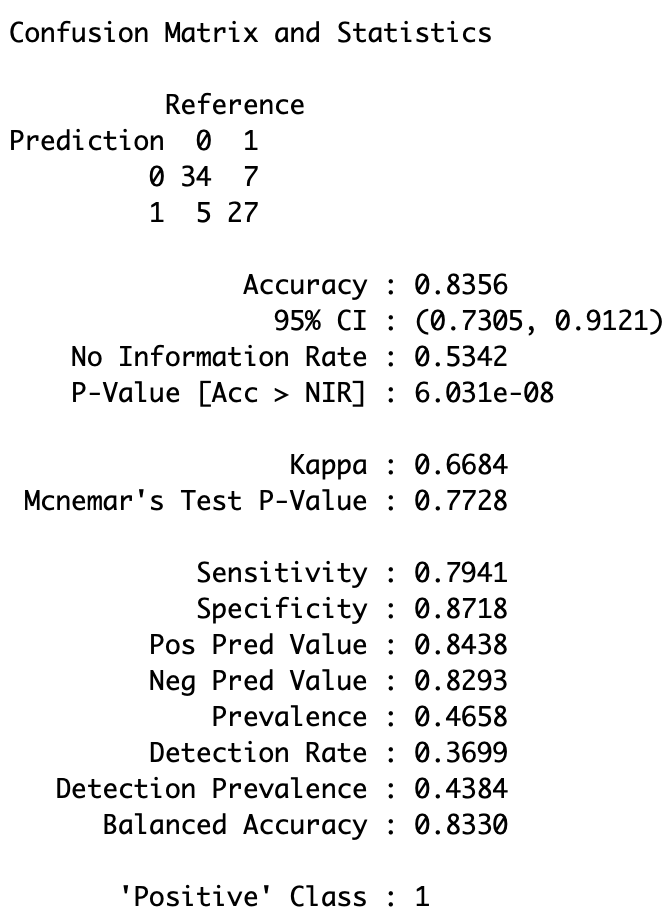
\includegraphics[width=0.9\textwidth]{ThesisTemplate/appendix/images/Chapter5Appendix/ConfusionMatrix75/HA.png}
        \caption{Confusion Matrix output for Random Forest fitted to the Heart Attack Dataset after under-sampling (75\% majority class retained)}
        \label{fig:matrixHA75}
    \end{minipage}
\end{figure}

\begin{figure}[!htbp]
    \centering
    \begin{minipage}{0.45\textwidth}
        \centering
        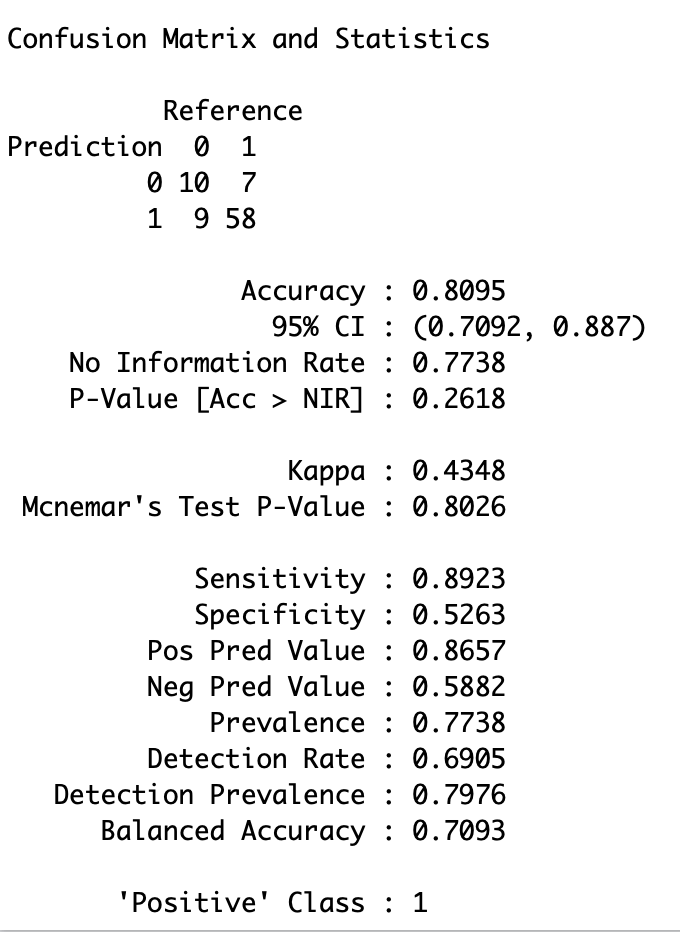
\includegraphics[width=0.9\textwidth]{ThesisTemplate/appendix/images/Chapter5Appendix/ConfusionMatrix75/LBP.png}
        \caption{Confusion Matrix output for Random Forest fitted to the Low Back Pain Dataset after under-sampling (75\% majority class retained)}
        \label{fig:matrixLBP75}
    \end{minipage}\hfill
    \begin{minipage}{0.45\textwidth}
        \centering
        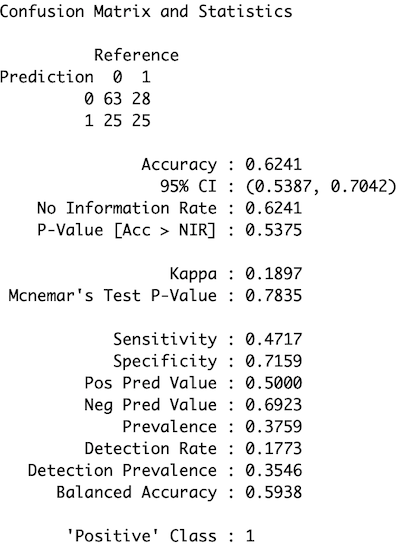
\includegraphics[width=0.9\textwidth]{ThesisTemplate/appendix/images/Chapter5Appendix/ConfusionMatrix75/Liver.png}
        \caption{Confusion Matrix output for Random Forest fitted to the Liver Dataset after under-sampling (75\% majority class retained)}
        \label{fig:matrixLiver75}
    \end{minipage}
\end{figure}

\begin{figure}[!htbp]
    \centering
    \begin{minipage}{0.45\textwidth}
        \centering
        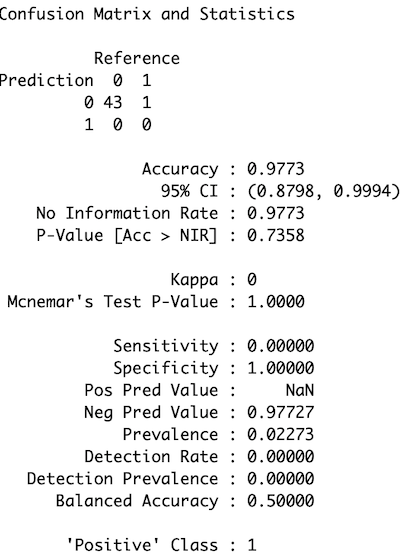
\includegraphics[width=0.9\textwidth]{ThesisTemplate/appendix/images/Chapter5Appendix/ConfusionMatrix75/ModifiedHA.png}
        \caption{Confusion Matrix output for Random Forest fitted to the Modified Heart Attack Dataset after under-sampling (75\% majority class retained)}
        \label{fig:matrixmodHA75}
    \end{minipage}\hfill
    \begin{minipage}{0.45\textwidth}
        \centering
        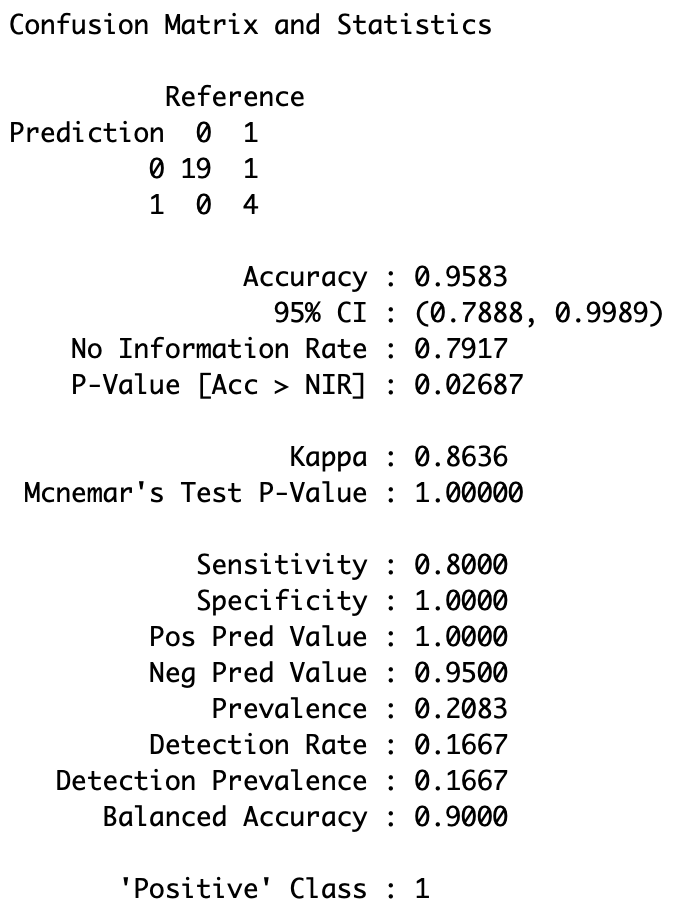
\includegraphics[width=0.9\textwidth]{ThesisTemplate/appendix/images/Chapter5Appendix/ConfusionMatrix75/ModifiedLBP.png}
        \caption{Confusion Matrix output for Random Forest fitted to the Modified Low Back Pain Dataset after under-sampling (75\% majority class retained)}
        \label{fig:matrixmodLBP75}
    \end{minipage}
\end{figure}

\begin{figure}[!htbp]
    \centering
    \begin{minipage}{0.45\textwidth}
        \centering
        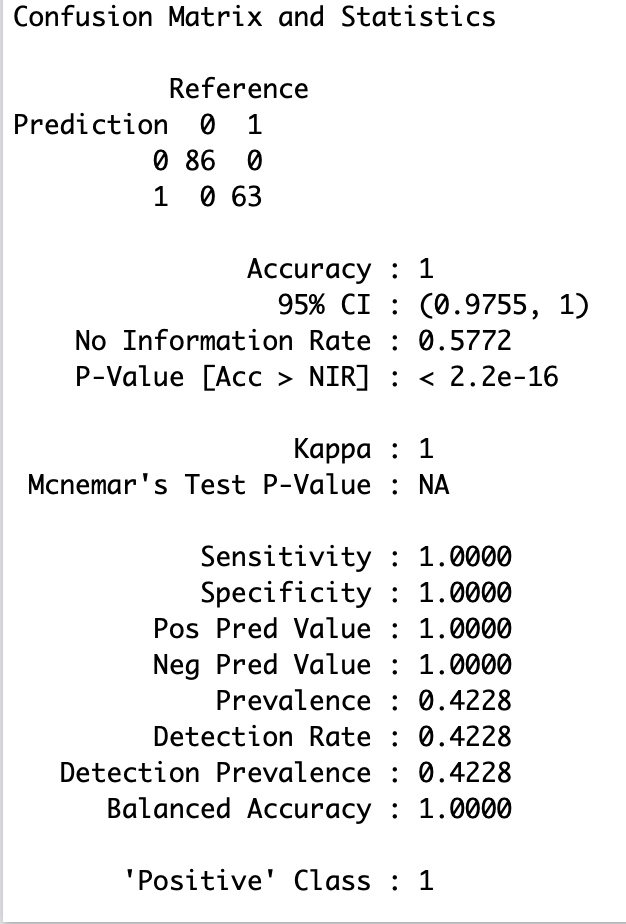
\includegraphics[width=0.9\textwidth]{ThesisTemplate/appendix/images/Chapter5Appendix/ConfusionMatrix60/Autism.png}
        \caption{Confusion Matrix output for Random Forest fitted to the Autism Dataset after under-sampling (60\% majority class retained)}
        \label{fig:matrixAutism60}
    \end{minipage}\hfill
    \begin{minipage}{0.45\textwidth}
        \centering
        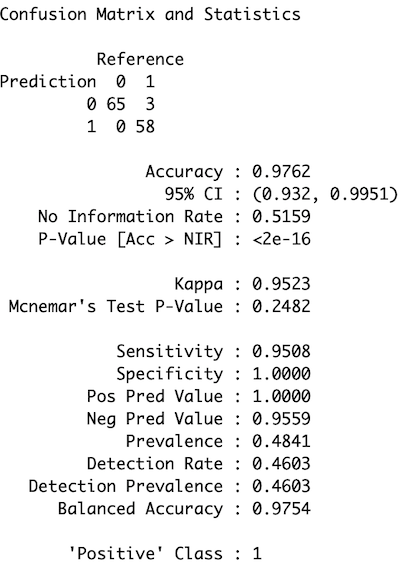
\includegraphics[width=0.9\textwidth]{ThesisTemplate/appendix/images/Chapter5Appendix/ConfusionMatrix60/BreastCancer.png}
        \caption{Confusion Matrix output for Random Forest fitted to the Breast Cancer Dataset after under-sampling (60\% majority class retained)}
        \label{fig:matrixBC60}
    \end{minipage}
\end{figure}

\begin{figure}[!htbp]
    \centering
    \begin{minipage}{0.45\textwidth}
        \centering
        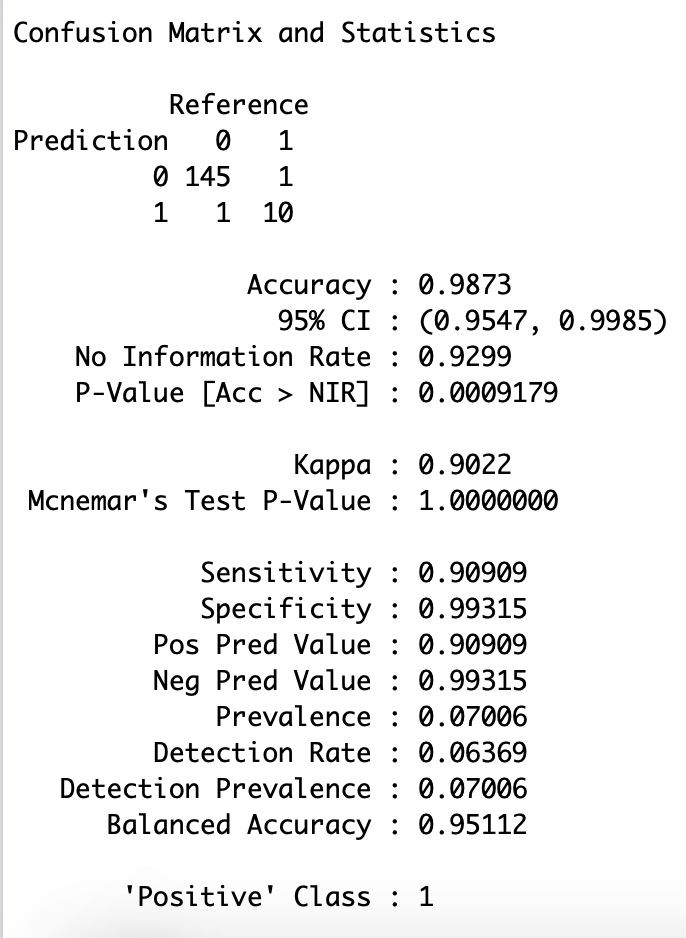
\includegraphics[width=0.9\textwidth]{ThesisTemplate/appendix/images/Chapter5Appendix/ConfusionMatrix60/CervicalCancer.png}
        \caption{Confusion Matrix output for Random Forest fitted to the Cervical Cancer after under-sampling (60\% majority class retained)}
        \label{fig:matrixCC60}
    \end{minipage}\hfill
    \begin{minipage}{0.45\textwidth}
        \centering
        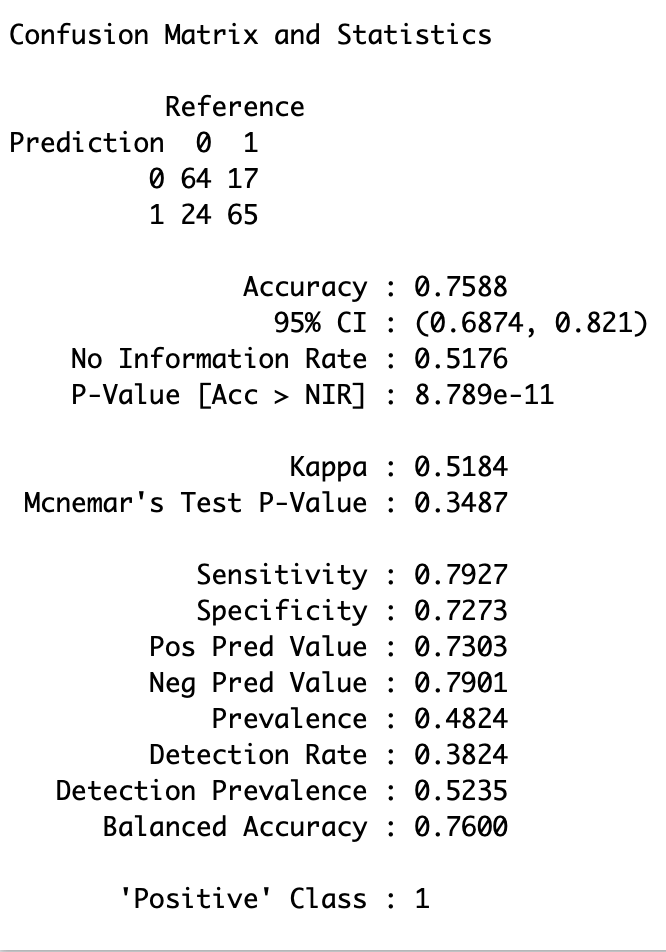
\includegraphics[width=0.9\textwidth]{ThesisTemplate/appendix/images/Chapter5Appendix/ConfusionMatrix60/Diabetes.png}
        \caption{Confusion Matrix output for Random Forest fitted to the Diabetes Dataset after under-sampling (60\% majority class retained)}
        \label{fig:matrixDia60}
    \end{minipage}
\end{figure}

\begin{figure}[!htbp]
    \centering
    \begin{minipage}{0.45\textwidth}
        \centering
        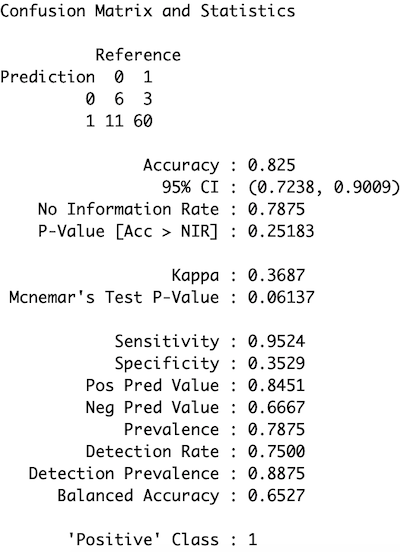
\includegraphics[width=0.9\textwidth]{ThesisTemplate/appendix/images/Chapter5Appendix/ConfusionMatrix60/LBP.png}
        \caption{Confusion Matrix output for Random Forest fitted to the Low Back Pain Dataset after under-sampling (60\% majority class retained)}
        \label{fig:matrixLBP60}
    \end{minipage}\hfill
    \begin{minipage}{0.45\textwidth}
        \centering
        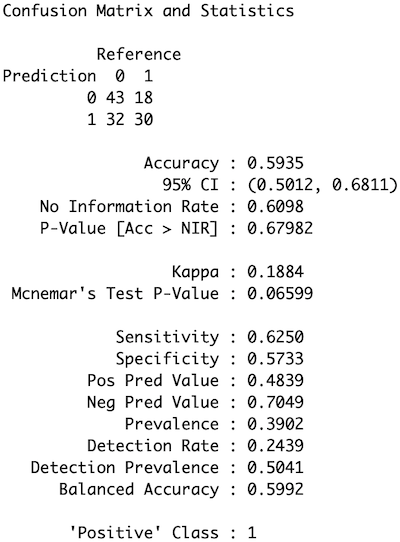
\includegraphics[width=0.9\textwidth]{ThesisTemplate/appendix/images/Chapter5Appendix/ConfusionMatrix60/Liver.png}
        \caption{Confusion Matrix output for Random Forest fitted to the Liver Dataset after under-sampling (60\% majority class retained)}
        \label{fig:matrixLiver60}
    \end{minipage}
\end{figure}

\begin{figure}[!htbp]
    \centering
    \begin{minipage}{0.45\textwidth}
        \centering
        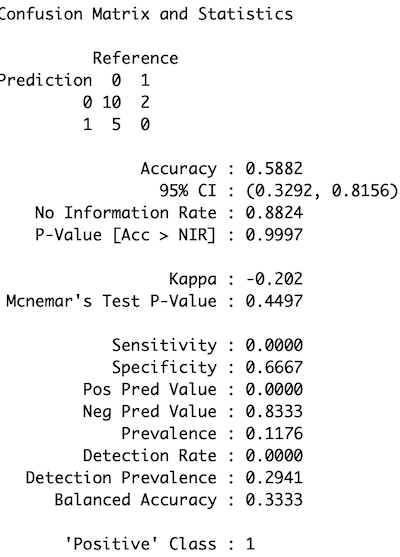
\includegraphics[width=0.9\textwidth]{ThesisTemplate/appendix/images/Chapter5Appendix/ConfusionMatrix60/Fertility.png}
        \caption{Confusion Matrix output for Random Forest fitted to the Fertility Dataset after under-sampling (60\% majority class retained)}
        \label{fig:matrixFert60}
    \end{minipage}\hfill
    \begin{minipage}{0.45\textwidth}
        \centering
        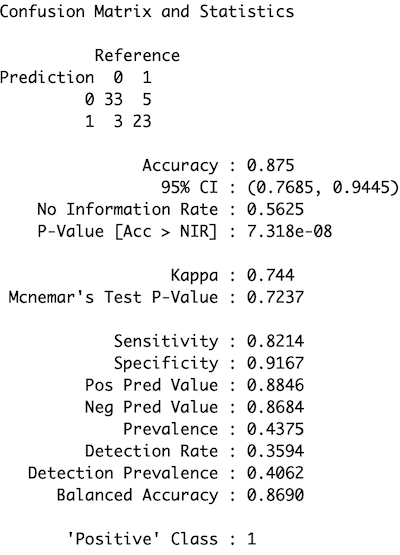
\includegraphics[width=0.9\textwidth]{ThesisTemplate/appendix/images/Chapter5Appendix/ConfusionMatrix60/HA.png}
        \caption{Confusion Matrix output for Random Forest fitted to the Heart Attack Dataset after under-sampling (60\% majority class retained)}
        \label{fig:matrixHA60}
    \end{minipage}
\end{figure}

\begin{figure}[!htbp]
    \centering
    \begin{minipage}{0.45\textwidth}
        \centering
        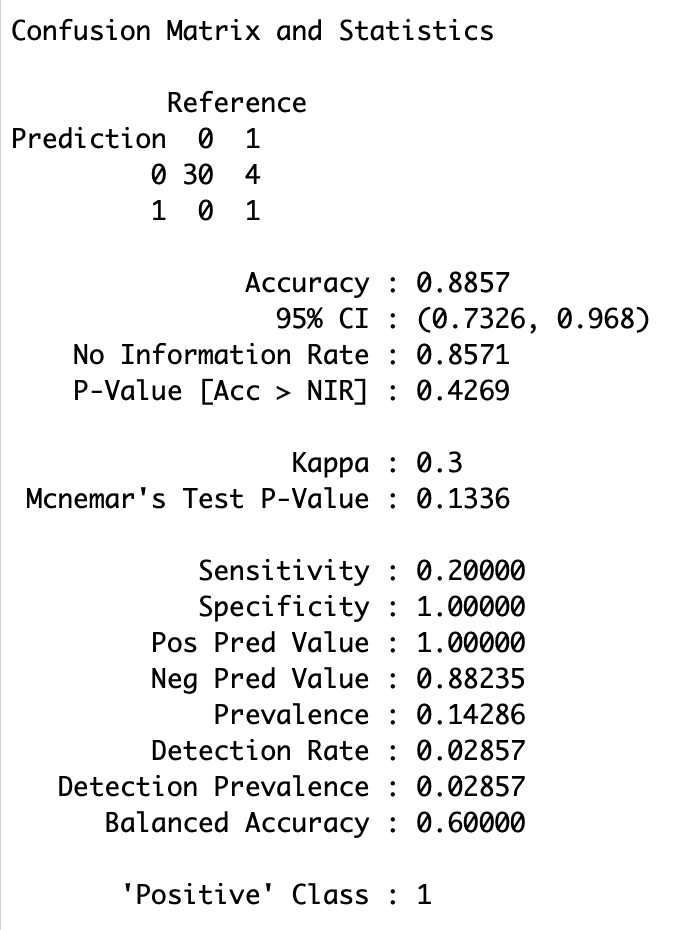
\includegraphics[width=0.9\textwidth]{ThesisTemplate/appendix/images/Chapter5Appendix/ConfusionMatrix60/modHA.png}
        \caption{Confusion Matrix output for Random Forest fitted to the Modified Heart Attack Dataset after under-sampling (60\% majority class retained)}
        \label{fig:matrixmodHA60}
    \end{minipage}\hfill
    \begin{minipage}{0.45\textwidth}
        \centering
        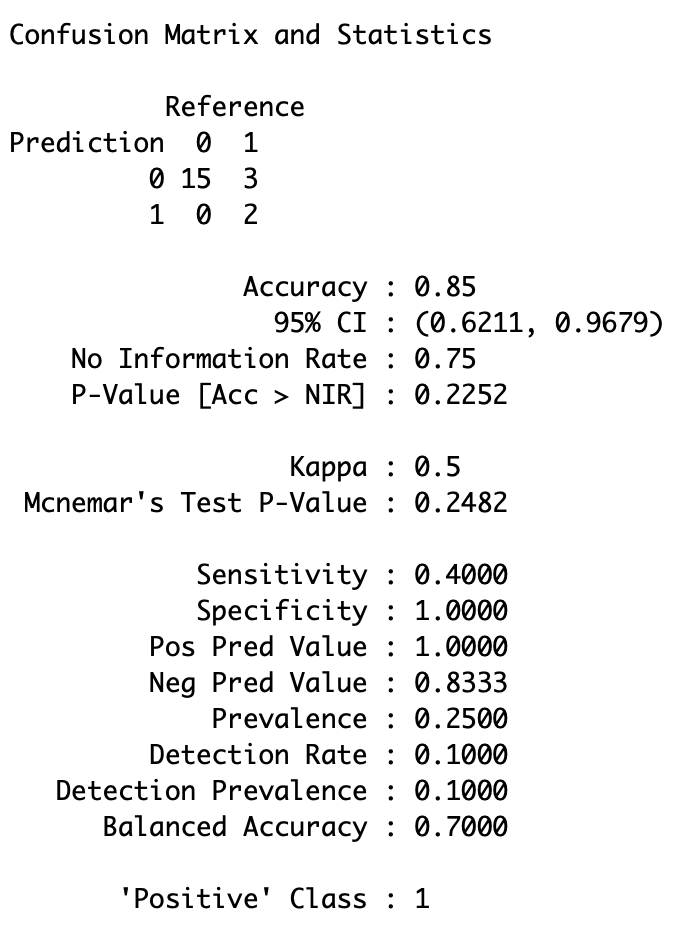
\includegraphics[width=0.9\textwidth]{ThesisTemplate/appendix/images/Chapter5Appendix/ConfusionMatrix60/modLBP.png}
        \caption{Confusion Matrix output for Random Forest fitted to the Modified Low Back Pain Dataset after under-sampling (60\% majority class retained)}
        \label{fig:matrixmodLBP60}
    \end{minipage}
\end{figure}

\begin{figure}[!htbp]
    \centering
    \begin{minipage}{0.45\textwidth}
        \centering
        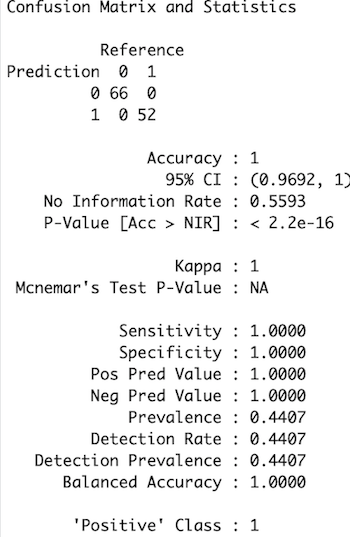
\includegraphics[width=0.9\textwidth]{ThesisTemplate/appendix/images/Chapter5Appendix/ConfusionMatrix40/Autism.png}
        \caption{Confusion Matrix output for Random Forest fitted to the Autism Dataset after under-sampling (40\% majority class retained)}
        \label{fig:matrixAutism40}
    \end{minipage}\hfill
    \begin{minipage}{0.45\textwidth}
        \centering
        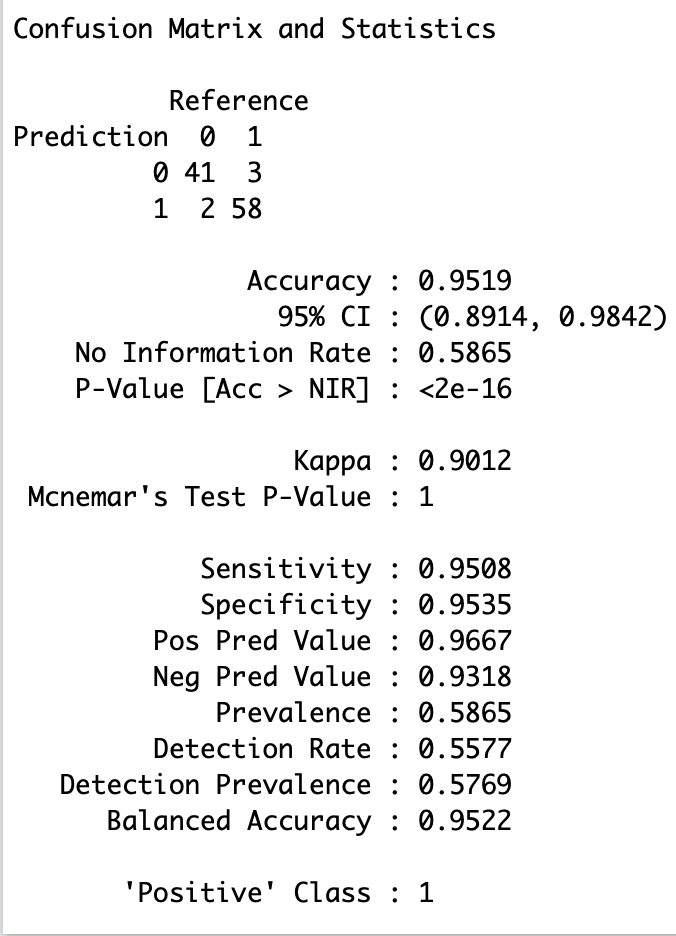
\includegraphics[width=0.9\textwidth]{ThesisTemplate/appendix/images/Chapter5Appendix/ConfusionMatrix40/BreastCancer.png}
        \caption{Confusion Matrix output for Random Forest fitted to the Breast Cancer Dataset after under-sampling (40\% majority class retained)}
        \label{fig:matrixBC40}
    \end{minipage}
\end{figure}

\begin{figure}[!htbp]
    \centering
    \begin{minipage}{0.45\textwidth}
        \centering
        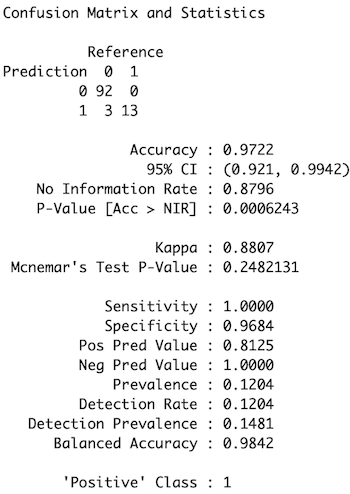
\includegraphics[width=0.9\textwidth]{ThesisTemplate/appendix/images/Chapter5Appendix/ConfusionMatrix40/CervicalCancer.png}
        \caption{Confusion Matrix output for Random Forest fitted to the Cervical Cancer Dataset after under-sampling (40\% majority class retained)}
        \label{fig:matrixCC40}
    \end{minipage}\hfill
    \begin{minipage}{0.45\textwidth}
        \centering
        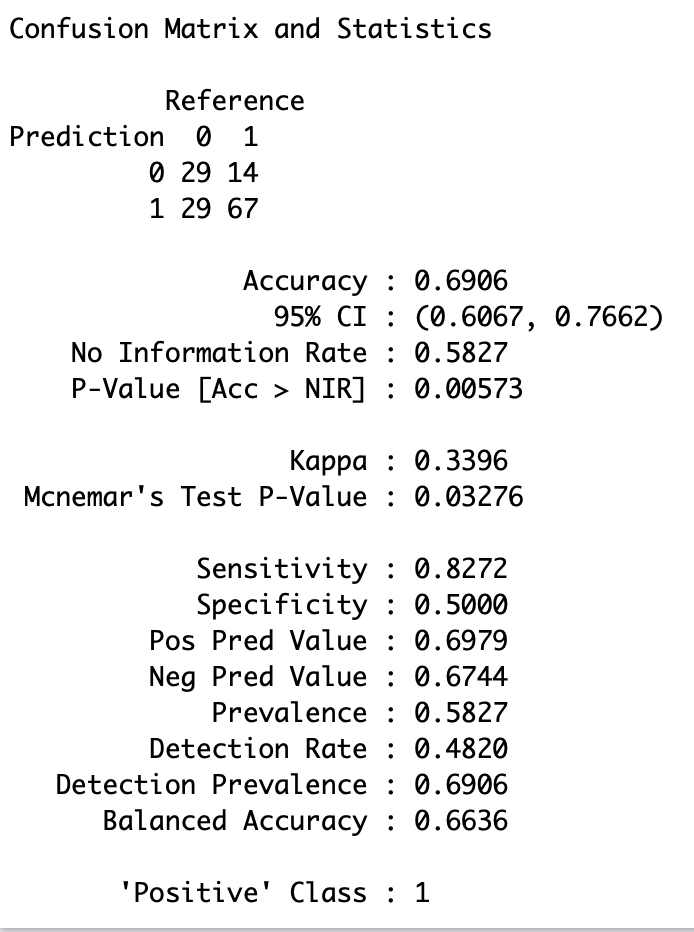
\includegraphics[width=0.9\textwidth]{ThesisTemplate/appendix/images/Chapter5Appendix/ConfusionMatrix40/Diabetes.png}
        \caption{Confusion Matrix output for Random Forest fitted to the Diabetes Dataset after under-sampling (40\% majority class retained)}
        \label{fig:matrixDia40}
    \end{minipage}
\end{figure}

\begin{figure}[!htbp]
    \centering
    \begin{minipage}{0.45\textwidth}
        \centering
        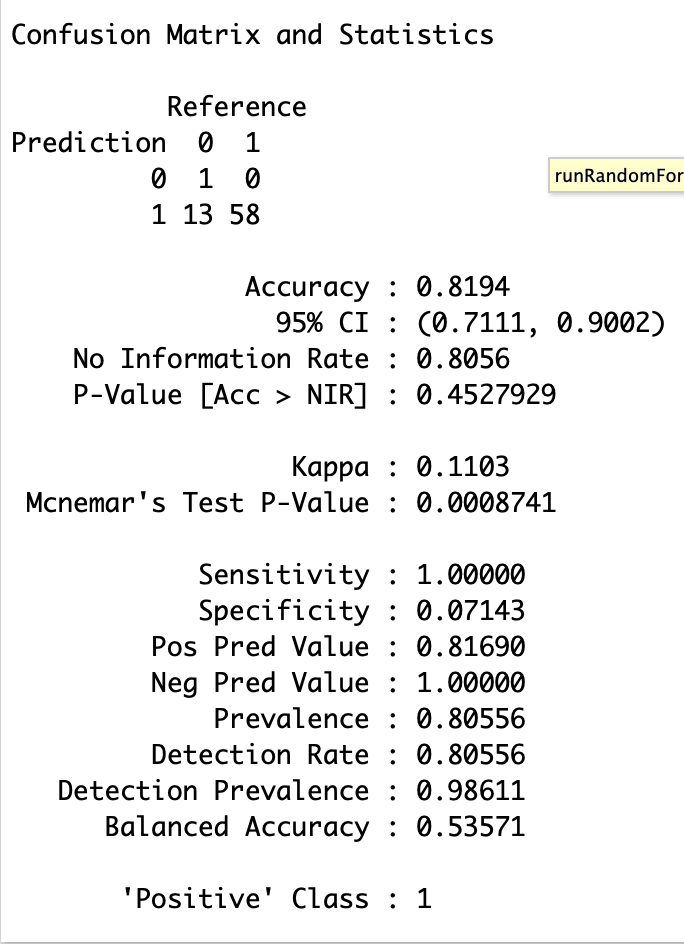
\includegraphics[width=0.9\textwidth]{ThesisTemplate/appendix/images/Chapter5Appendix/ConfusionMatrix40/LBP.png}
        \caption{Confusion Matrix output for Random Forest fitted to the Low Back Pain Dataset after under-sampling (40\% majority class retained)}
        \label{fig:matrixLBP40}
    \end{minipage}\hfill
    \begin{minipage}{0.45\textwidth}
        \centering
        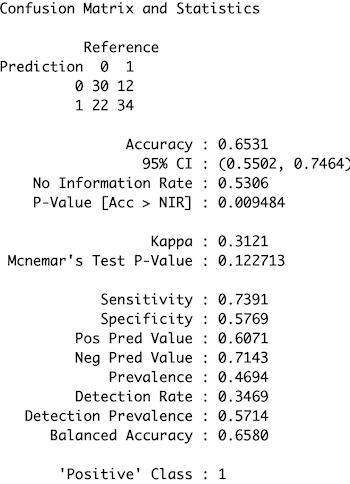
\includegraphics[width=0.9\textwidth]{ThesisTemplate/appendix/images/Chapter5Appendix/ConfusionMatrix40/Liver.png}
        \caption{Confusion Matrix output for Random Forest fitted to the Liver Dataset after under-sampling (40\% majority class retained)}
        \label{fig:matrixLiver40}
    \end{minipage}
\end{figure}

\begin{figure}[!htbp]
    \centering
    \begin{minipage}{0.45\textwidth}
        \centering
        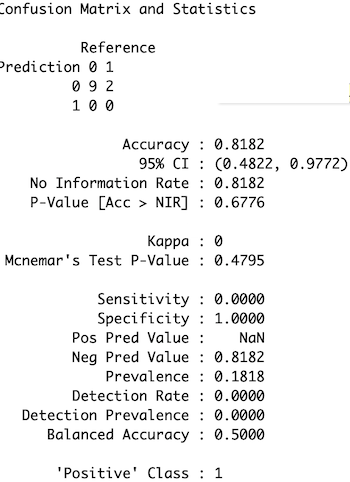
\includegraphics[width=0.9\textwidth]{ThesisTemplate/appendix/images/Chapter5Appendix/ConfusionMatrix40/Fertility.png}
        \caption{Confusion Matrix output for Random Forest fitted to the Fertility Dataset after under-sampling (40\% majority class retained)}
        \label{fig:matrixFert40}
    \end{minipage}\hfill
    \begin{minipage}{0.45\textwidth}
        \centering
        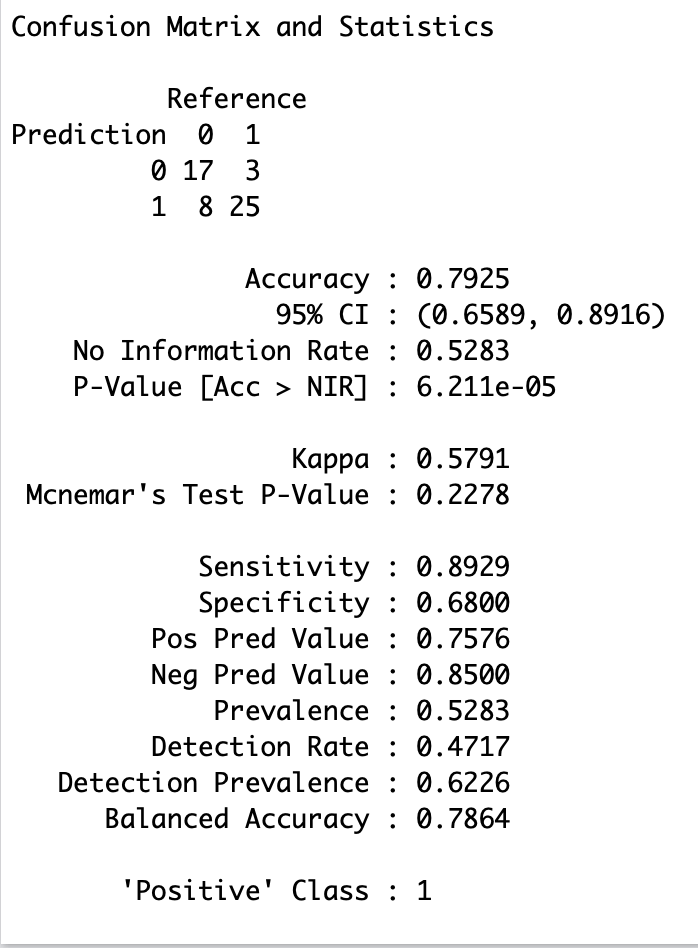
\includegraphics[width=0.9\textwidth]{ThesisTemplate/appendix/images/Chapter5Appendix/ConfusionMatrix40/HA.png}
        \caption{Confusion Matrix output for Random Forest fitted to the Heart Attack Dataset after under-sampling (40\% majority class retained)}
        \label{fig:matrixHA40}
    \end{minipage}
\end{figure}

\begin{figure}[!htbp]
    \centering
    \begin{minipage}{0.45\textwidth}
        \centering
        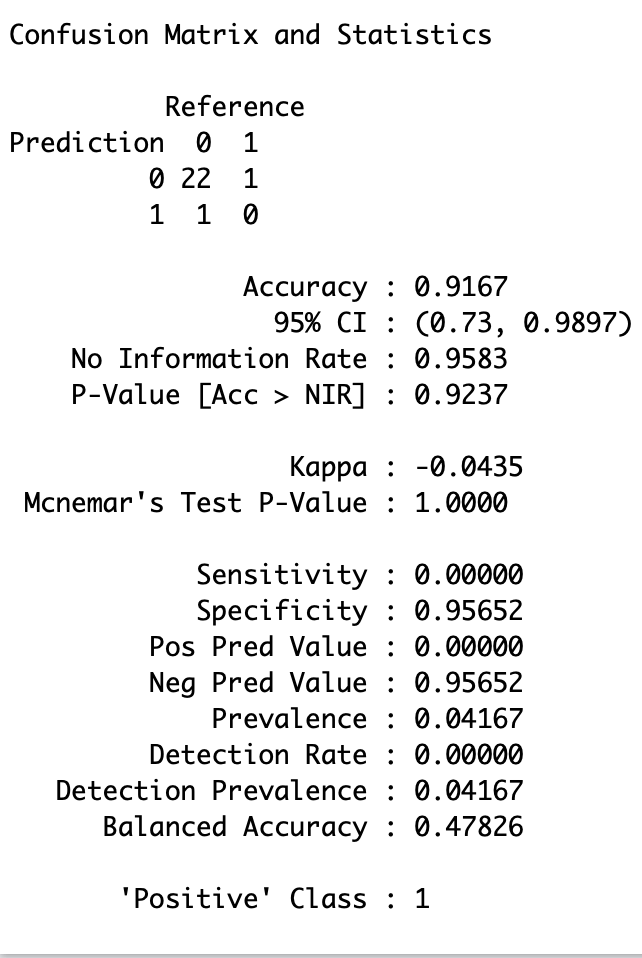
\includegraphics[width=0.9\textwidth]{ThesisTemplate/appendix/images/Chapter5Appendix/ConfusionMatrix40/modHA.png}
        \caption{Confusion Matrix output for Random Forest fitted to the Modified Heart Attack Dataset after under-sampling (40\% majority class retained)}
        \label{fig:matrixmodHA40}
    \end{minipage}\hfill
    \begin{minipage}{0.45\textwidth}
        \centering
        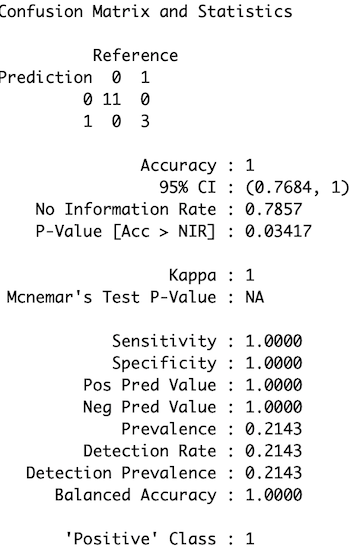
\includegraphics[width=0.9\textwidth]{ThesisTemplate/appendix/images/Chapter5Appendix/ConfusionMatrix40/modLBP.png}
        \caption{Confusion Matrix output for Random Forest fitted to the Modified Low Back Pain Dataset after under-sampling (40\% majority class retained)}
        \label{fig:matrixmodLBP40}
    \end{minipage}
\end{figure}


\begin{table}[ht]
\centering
\begin{tabular}{lrrr}
  \hline
  \rowcolor{LightCyan}
Dataset & Variation75 & Variation60 & Variation40 \\ 
  \hline
AuSDf & 0.00 & 0.00 & 0.00 \\ 
  BCDf & -0.04 & 0.06 & 0.04 \\ 
  CCDf & -0.00 & -0.01 & -0.02 \\ 
  DiabetesDf & 0.02 & 0.02 & -0.05 \\ 
  FertDf & -0.02 & -0.34 & -0.11 \\ 
  HAPDf & -0.07 & -0.03 & -0.12 \\ 
  LBPDf & -0.01 & 0.01 & 0.00 \\ 
  LiverDf & -0.09 & -0.12 & -0.06 \\ 
  subHAPDf & 0.03 & -0.06 & -0.03 \\ 
  subLBPDf & 0.05 & -0.06 & 0.09 \\ 
   \hline
\end{tabular}
\caption{Observed variations in accuracy for all datasets for the three different conditions of under-sampling}
\label{tab:variationsAccu}
\end{table}

\begin{table}[ht]
\centering
\begin{tabular}{lrrr}
  \hline
   \rowcolor{LightCyan}
Dataset & Variation75 & Variation60 & Variation40 \\ 
  \hline
AuSDf & 0.00 & 0.00 & 0.00 \\ 
  BCDf & 0.06 & 0.10 & 0.10 \\ 
  CCDf & 0.00 & 0.01 & 0.10 \\ 
  DiabetesDf & 0.14 & 0.24 & 0.27 \\ 
  FertDf & 0.33 & 0.00 & 0.00 \\ 
  HAPDf & -0.04 & -0.01 & 0.06 \\ 
  LBPDf & -0.01 & 0.05 & 0.10 \\ 
  LiverDf & 0.12 & 0.27 & 0.39 \\ 
  subHAPDf & 0.00 & 0.20 & 0.00 \\ 
  subLBPDf & 0.30 & -0.10 & 0.50 \\ 
   \hline
\end{tabular}
\caption{Observed variations in sensitivity for all datasets for the three different conditions of under-sampling}
\label{tab:variationsSensi}
\end{table}

\begin{table}[ht]
\centering
\begin{tabular}{lrrr}
  \hline
  \rowcolor{LightCyan}
Dataset & Variation75 & Variation60 & Variation40 \\ 
  \hline
AuSDf & 0.00 & 0.00 & 0.00 \\ 
  BCDf & -0.13 & 0.06 & 0.03 \\ 
  CCDf & 0.00 & -0.09 & -0.19 \\ 
  DiabetesDf & 0.02 & 0.01 & -0.03 \\ 
  FertDf &  &  &  \\ 
  HAPDf & -0.05 & -0.01 & -0.14 \\ 
  LBPDf & 0.03 & 0.01 & -0.02 \\ 
  LiverDf & -0.08 & -0.09 & 0.03 \\ 
  subHAPDf &  & 1.00 & 0.00 \\ 
  subLBPDf & 0.00 & 0.00 & 0.00 \\ 
   \hline
\end{tabular}
\caption{Observed variations in precision for all datasets for the three different conditions of under-sampling}
\label{tab:variationsPreci}
\end{table}

\begin{table}[ht]
\centering
\begin{tabular}{lrrr}
  \hline
  \rowcolor{LightCyan}
Dataset & Variation75 & Variation60 & Variation40 \\ 
  \hline
AuSDf & 0.00 & 0.00 & 0.00 \\ 
  BCDf & -0.04 & 0.08 & 0.06 \\ 
  CCDf & 0.00 & -0.04 & -0.05 \\ 
  DiabetesDf & 0.09 & 0.13 & 0.13 \\ 
  FertDf &  &  &  \\ 
  HAPDf & -0.04 & -0.01 & -0.04 \\ 
  LBPDf & 0.01 & 0.03 & 0.03 \\ 
  LiverDf & 0.05 & 0.11 & 0.23 \\ 
  subHAPDf &  &  &  \\ 
  subLBPDf & 0.22 & -0.10 & 0.33 \\ 
   \hline
\end{tabular}
\caption{Observed variations in F1 score for all datasets for the three different conditions of under-sampling}
\label{tab:variationsF1}
\end{table}


\begin{table}[ht]
\centering
\begin{tabular}{lrrrr}
  \hline
  \rowcolor{LightCyan}
Dataset & AccuVariation & SensiVariation & PreciVariation & F1Variation \\ 
  \hline
AuSDf & 0.00 & 0.00 & 0.00 & 0.00 \\ 
  BCDf & 0.01 & 0.04 & -0.01 & 0.02 \\ 
  CCDf & -0.02 & 0.00 & -0.36 & -0.20 \\ 
  DiabetesDf & 0.00 & 0.01 & 0.00 & 0.01 \\ 
  HAPDf & -0.03 & -0.03 & -0.07 & -0.05 \\ 
  LBPDf & 0.02 & -0.05 & 0.06 & 0.01 \\ 
  LiverDf & -0.03 & 0.07 & -0.08 & 0.02 \\ 
  subHAPDf & 0.00 & 0.67 & 0.50 &  \\ 
  subLBPDf & -0.16 & 0.00 & -0.75 & -0.33 \\ 
  FertDf & -0.21 & 0.50 &  &  \\ 
   \hline
\end{tabular}
\caption{Observed variations in performance metrics after SMOTE was applied to the training set compared to the baseline set in experiment 1}
\label{tab:variationsSMOTE}
\end{table}
 

\chapter{Project Log}

\begin{table}[ht]
    \centering
    \begin{tabular}{lrr}
    \hline
    \rowcolor{LightCyan}
       Week  & Date & Topic  \\
       0    &  17/09    &  Initial Meeting - project overview     \\
       1    &  26/09    &  Research - Project proposal writing \\
       2    &  2/10     & Discussion of Project proposal submission \\
       3    &  9/10     & literature review research and writing, early draft\\
       4    & 16/10     & Literature review writing\\
       5    & 23/10     & Literature review writing and researching \\
       6    & 29/10     & feedback  on first draft of lit. review  \\
       7    & 6/11      & adjustments to first draft/ submission of lit review \\
       8    & 13/11     & project requirement decisions and discussion      \\
       9    & 19/11     & project requirement write up/first draft      \\
       10   & 26/11     & project requirement adjustments/ writing/submission\\
       
    \end{tabular}
    \caption{Semester 1}
    \label{tab:proj_log1}
\end{table}


\begin{table}[ht]
    \centering
    \begin{tabular}{lrr}
    \hline
    \rowcolor{LightCyan}
       Week  & Date & Topic  \\
       0     & 8/01     &  Exploratory Data Analysis      \\
       0     & 15/01    &  Exploratory Data Analysis - Meeting    \\
       0     & 22/01    &  Initial Fit for RF Exploratory Data Analysis\\
       1     & 29/10    &  Redo fit on RF - rewrite code - some errors \\
       2     &  5/02    &  Add code to output metrics      \\
       3     &  12/02   & Change to EDA - repeat experiments  \\
       4     &  19/02   & Under-sampling- more EDA changes - reduce factor levels  \\
       5     &  26/02   & SMOTE first attempts    \\
       6     &  5/03    & Repeat SMOTE experiments - performed on both test and train      \\
       7     &  12/03   & Repeat SMOTE with better parameters for some of the datasets   \\
       8     &  19/03   & Final SMOTE experiment - final script   \\
       9    `&  26/03   & Supporting Graphs for data    \\
       10    &  9/04    & Thesis writing - Chapter 4 + poster   \\
       11    &  16/04   & Thesis writing + poster submission + additional graphs generated    \\
       12    &  23/04   & Thesis writing + checking   \\
       
    \end{tabular}
    \caption{Semester 2}
    \label{tab:proj_log2}
\end{table}



\chapter{GitHub Repository ReadMe}
https://github.com/AMacleod79/HonoursProjectCode


HonoursProjectCode ReadMe

This is a repository to back up and version control all of the code for my honours project.
This is a collection of  R-studio notebooks. The notebooks correspond to each project in the repository.
The R scripts should be used to run experiments and can be reused for different datasets (as long as label is in the last column).


 --Disregard -- Notebooks were used at the beginning but found to be impractical -- List of notebooks:

-  DataExploration.Rmd
- InitialDataModelling.Rmd

 List of EDA R scripts
- AutismEDA.R
- BreastCancerEDA.R
- CervicalcancerEDA.R
- ClassDist.R
- DiabetesEDA.R
- FertilityEDA.R
- HeartAttackEDA.R
- LiverDataEDA.R
- LowBackPainEDA.R

 List of csv files -- pre-processed data
 - BCDf.csv
 - LiverDf.csv
 - DiabetesDf.csv
 - AuSDf.csv
 - HAPDf.csv
 - LBPDf.csv
 - CCDf.csv
 - FertDf.csv
 - AlzDf.csv
 
List of R scripts
 - DatasetUploads.R
 - Train\_Test\_Split.R
 - RandomForestModelling.R
 - OverUnderSampling.R
 - RandomForestModellingSmote.R
 - LatexTable.R
 - SMOTEALL.R
 - SMOTEOne.R
 
 List of Experiments
 
 - Experiment1.R
 - Experiment2.R
 - Experiment3.R
 
 List of graph generating scripts
 - GroupedGraphs.R
 - VariationsGraph.R
 - GraphCreator.R
 - OverSamplingGraphs.R
 
 Notes
Please disregard the .rda files as they do not upload properly on R studio

